%%%% Document setup
\documentclass[a4paper,landscape,title page]{article}
\setlength{\oddsidemargin}{-0.65in}	% default=0in
\setlength{\textwidth}{11in}		% default=9in
\setlength{\textheight}{6.85in}		% default=5.15in
\setlength{\topmargin}{-1.0in}		% default=0.20in
\setlength{\headsep}{0.35in}		% default=0.35in
\setlength{\parskip}{1.2ex}
\setlength{\parindent}{0mm}

%%%% Use packages
\usepackage{times}
\usepackage{tikz,pgf}
\usetikzlibrary{arrows,automata,trees,plotmarks,calc}


%%%%
\title{Goal-Plan hierarchy for test \textit{testImpactvars3}}
\author{
Dhirendra Singh\\
dhirendra.singh@rmit.edu.au}
\begin{document}
\maketitle

\begin{figure*}[t]
\begin{center}

\begin{tikzpicture}[scale=1.5,level distance=1.2cm]
\tikzstyle{txt}=[scale=1.1]
\tikzstyle{planbox}=[scale=1.1,draw,minimum height=0.7cm,minimum width=1.1cm]
\tikzstyle{goalbox}=[scale=1.1,draw,rounded corners,minimum height=0.7cm,minimum width=1.1cm]
\tikzstyle{level 1}=[sibling distance=6cm] 
\tikzstyle{level 2}=[sibling distance=8cm] 
\tikzstyle{level 3}=[sibling distance=4.0cm]
\tikzstyle{level 4}=[sibling distance=2.0cm]
\tikzstyle{level 5}=[sibling distance=1cm]

\node[goalbox,yshift=1cm,solid] (T) {$G$}
	child[dashed] {node[planbox] (P1) {$P_1$}}
	child[solid] {node[planbox] (Pi) {$P_i$}
		child {node[goalbox] {$G_{ia}$}
			child {node[planbox] {$P_{ia1}$}
				child {node[goalbox] {$G_{ia1a}$}
					child {node[planbox] {$P_{ia1aj}$} node[txt,below=0.3cm] {$\surd$}}
					child {node[planbox] {$P_{ia1a*}$} node[txt,below=0.3cm] {$\times$}
						edge from parent node[txt,right,near start] {$\times 2$}
					}
				}
				child {node[goalbox] {$G_{ia1b}$}
					child {node[planbox] {$P_{ia1bj}$} node[txt,below=0.3cm] {$\surd$}}
					child {node[planbox] {$P_{ia1b*}$} node[txt,below=0.3cm] {$\times$}
						edge from parent node[txt,right,near start] {$\times 2$}
					}
				}
			}
			child {node[planbox] {$P_{ia2}$}
				child {node[goalbox] {$G_{ia2a}$}
					child {node[planbox] {$P_{ia2aj}$} node[txt,below=0.3cm] {$\times$}}
					child {node[planbox] {$P_{ia2a*}$} node[txt,below=0.3cm] {$\times$}
						edge from parent node[txt,right,near start] {$\times 2$}
					}
				}
				child {node[goalbox] {$G_{ia2b}$}
					child {node[planbox] {$P_{ia2bj}$} node[txt,below=0.3cm] {$\times$}}
					child {node[planbox] {$P_{ia2b*}$} node[txt,below=0.3cm] {$\times$}
						edge from parent node[txt,right,near start] {$\times 2$}
					}
				}
			}
		}
		child {node[goalbox] {$G_{ib}$}
			child {node[planbox] {$P_{ib1}$}
				child {node[goalbox] {$G_{ib1a}$}
					child {node[planbox] {$P_{ib1aj}$} node[txt,below=0.3cm] {$\surd$}}
					child {node[planbox] {$P_{ib1a*}$} node[txt,below=0.3cm] {$\times$}
						edge from parent node[txt,right,near start] {$\times 2$}
					}
				}
				child {node[goalbox] {$G_{ib1b}$}
					child {node[planbox] {$P_{ib1bj}$} node[txt,below=0.3cm] {$\surd$}}
					child {node[planbox] {$P_{ib1b*}$} node[txt,below=0.3cm] {$\times$}
						edge from parent node[txt,right,near start] {$\times 2$}
					}
				}
			}
			child {node[planbox] {$P_{ib2}$}
				child {node[goalbox] {$G_{ib2a}$}
					child {node[planbox] {$P_{ib2aj}$} node[txt,below=0.3cm] {$\times$}}
					child {node[planbox] {$P_{ib2a*}$} node[txt,below=0.3cm] {$\times$}
						edge from parent node[txt,right,near start] {$\times 2$}
					}
				}
				child {node[goalbox] {$G_{ib2b}$}
					child {node[planbox] {$P_{ib2bj}$} node[txt,below=0.3cm] {$\times$}}
					child {node[planbox] {$P_{ib2b*}$} node[txt,below=0.3cm] {$\times$}
						edge from parent node[txt,right,near start] {$\times 2$}
					}
				}
			}
		}
	}
	child[dashed] {node[planbox] (P4) {$P_4$}}
;
\node[txt] at ($ (P1)!.5!(Pi) $) {$\ldots$};
\node[txt] at ($ (Pi)!.5!(P4) $) {$\ldots$};

\end{tikzpicture}

\vskip 1.5cm
\caption{Goal-Plan hierarchy for test \textit{testImpactvars3}. There are $2^3$ worlds whose solutions are distributed evenly in each of the $4$ top level plans. Successful execution trace is of length $4$. Within each sub-tree $P_i$ there is sufficient complexity but is not biased towards any approach. Overall both \textit{Stable} and \textit{Concurrent} perform comparably.}
\end{center}
\end{figure*}

\end{document}
%%%%